\documentclass{article}

\usepackage[italian]{babel}
\usepackage{crimson} % whole document font
\usepackage[T1]{fontenc}
\usepackage[utf8]{inputenc}
\usepackage{graphicx}
\usepackage{wrapfig}

\setlength{\parindent}{0pt}

\usepackage[a4paper]{geometry}
\geometry{
	top=3.25cm, % Top margin
	bottom=4cm, % Bottom margin
	left=3cm, % Left margin
	right=3cm, % Right margin
	headheight=0.75cm, % Header height
	footskip=1cm, % Space from the bottom margin to the baseline of the footer
	headsep=0.75cm, % Space from the top margin to the baseline of the header
	%showframe, % Uncomment to show how the type block is set on the page
}

\newcommand{\years}[1]{{\large #1}\\}

\usepackage[usenames, dvipsnames]{xcolor} % Required for specifying colours by name
\usepackage[bookmarks, colorlinks, breaklinks]{hyperref} % Required for links

% Set link colours
\hypersetup{
	linkcolor=blue,
	citecolor=blue,
	filecolor=black,
	urlcolor=MidnightBlue
}

\hypersetup{
	pdftitle={Filippo Barbari - Curriculum vitae},
	pdfauthor={Filippo Barbari}
}

\newcommand{\referenza}[6]{
	\textbf{#1}
	\begin{itemize}
		\setlength\itemsep{0em}
		\item #2
		\item[-] Mail: #3
		\item[$\star$] Telefono: #4
		\item[$\circ$] Sito: #5
		\item[] \textit{#6}
	\end{itemize}
}

\newcommand{\https}[1]{\href{https://#1}{#1}}

\newcommand{\exam}[2]{\textbf{#1}\hfill \ifnum #2<31 {\Large #2}{\small /30} \else {\Large 30}{\small /30 con lode} \fi\\}

\newcommand{\skill}[2]{#1 #2/10}

\begin{document}
	
	\begin{wrapfigure}[0]{r}{0.2\textwidth}
		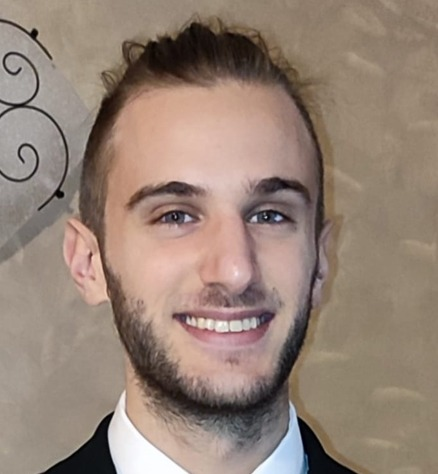
\includegraphics[width=0.18\textwidth]{fototessera}
	\end{wrapfigure}
		
	{\LARGE\bfseries Filippo Barbari} % Name
	\bigskip
	
	Via Emilia 42\\ % Address
	47838 Riccione (RN), Italia
	\medskip % Whitespace
	
	Telefono: +39 327 2207037\\
	Fisso: +39 0541 644233
	\medskip
	
	\noindent
	\begin{tabular}{ll}
		Email: & \href{mailto:filippo.barbari@gmail.com}{filippo.barbari@gmail.com}\\
		Email istituzionale: & \href{mailto:filippo.barbari@studio.unibo.it}{filippo.barbari@studio.unibo.it}
	\end{tabular}
	\medskip
	
	Nato: 24 agosto 1999, Rimini (RN), Italia\\ % Date of birth
	Nazionalità: Italiana % Nationality
	\medskip
	
	Conoscenza italiano: madrelingua\\
	Conoscenza inglese: FCE livello B-2
	
	\section*{Referenze}
	
	\referenza{Prof. Moreno Marzolla}
	{Professore associato del Dipartimento di Informatica - Scienza e Ingegneria (DISI), Università di Bologna, Italia.}
	{\href{mailto:moreno.marzolla@unibo.it}{moreno.marzolla@unibo.it}}
	{+39 0547 338861}
	{\https{www.moreno.marzolla.name}}
	{\textit{Il prof. Marzolla è stato il relatore della mia tesi di laurea triennale e il tutor del mio tirocinio curriculare.}}
	
	\section*{Formazione}
	\years{2013 - 2018} \textbf{Diploma di Maturità} conseguito con votazione 90/100 presso Liceo Scientifico A. Volta, Riccione (RN)\\
	
	\years{2018 - 2021} \textbf{Laurea Triennale} in Ingegneria e Scienze Informatiche conseguita con votazione 106/110 presso Alma Mater Studiorum Università di Bologna, Campus di Cesena in data 7 ottobre 2021\\
	
	\years{2021 - oggi} \textbf{Laurea Magistrale} in Ingegneria e Scienze Informatiche presso Alma Mater Studiorum Università di Bologna, Campus di Cesena
	
	\subsection*{Esami sostenuti durante il corso di laurea triennale}
	\begin{minipage}[t]{.47\textwidth}
		\exam{Algebra e Geometria}{26}
		\exam{Algoritmi e Strutture Dati}{31}
		\exam{Analisi Matematica}{27}
		\exam{Architetture degli Elaboratori}{29}
		\exam{Basi di Dati}{30}
		\exam{Computer Graphics}{28}
		\exam{Crittografia}{30}
		\exam{Fisica}{31}
		\exam{High-Performance Computing}{30}
		\exam{Ingegneria del software}{23}
		\exam{Matematica Discreta e Probabilità}{25}
	\end{minipage}
	\hfill
	\begin{minipage}[t]{.47\textwidth}
		\exam{Metodi Numerici}{22}
		\exam{Programmazione}{28}
		\exam{Programmazione ad Oggetti}{28}
		\exam{Programmazione di Applicazioni\\Data-Intensive}{27}
		\exam{Programmazione di Reti}{28}
		\exam{Reti di telecomunicazione}{23}
		\exam{Ricerca operativa}{26}
		\exam{Sistemi Operativi}{24}
		\exam{Tecnologie web}{24}
	\end{minipage}

	\subsection*{Tirocinio curriculare}
	Sviluppo e valutazione delle prestazioni di un'applicazione parallela per simulazioni tecnico-scientifiche.
	
	Tutor: Prof. Moreno Marzolla
	
	Lo scopo di questo tirocinio è stato lo sviluppo di una simulazione per il calcolo dell'impacchettamento ottimale di sfere rappresentanti particelle di carburante all'interno di un serbatoio cubico.
	
	\subsection*{Tesi di Laurea Triennale}
	Implementazione CUDA dell'algoritmo di Bellman-Ford.
	
	Relatore: Prof. Moreno Marzolla
	
	Progettazione, sviluppo e valutazione delle prestazioni di tre differenti implementazioni parallele dell'algoritmo di Bellman-Ford su GPU.
	
	Votazione finale: 106/110
	
	Link: \https{amslaurea.unibo.it/24313}
	
	Codice: \https{github.com/Ledmington/bellman-ford-cuda}
	
	\subsection*{Esami sostenuti durante il corso di laurea magistrale}
	{\small Ultimo aggiornamento: 27/01/2022}
	\medskip
	
	\begin{minipage}[t]{.47\textwidth}
		\exam{Machine Learning}{29}
	\end{minipage}
	\hfill
	\begin{minipage}[t]{.47\textwidth}
		% aggiungere qui futuri esami
	\end{minipage}
	
	\section*{Confidenza}
	\subsection*{Linguaggi di programmazione}
	\skill{C}{9}\\
	\skill{C++}{6}\\
	\skill{Java}{7}\\
	\skill{Bash}{4}
	
	\subsection*{Altri linguaggi}
	\skill{HTML}{9}\\
	\skill{MarkDown}{6}\\
	\skill{\LaTeX}{7}
	
	\subsection*{Software}
	\skill{Visual Studio}{9}\\
	\skill{Git}{6}\\
	\skill{GitHub Actions}{7}
	
	\section*{Altre attività}
	\years{2018} Ho partecipato agli allenamenti della squadra di Cesena del ACM ICPC.\\
	
	\years{2014} Ho raggiunto le fasi provinciali delle Olimpiadi di Matematica.
	
	\vfill
	\begin{center}
		\scriptsize
		Ultimo aggiornamento: \today
	\end{center}
	
\end{document}